\documentclass[12pt]{article}
\usepackage{graphicx}
\usepackage{amssymb}
  \usepackage{url,hyperref}
  \usepackage{epstopdf}
  \usepackage[usenames,dvipsnames]{color}
\usepackage{sidecap}
\usepackage{listings}
\usepackage{natbib}

%%%%%%%%%%%%%%%
% User defined macros
%%%%%%%%%%%%%%%

\newcommand{\apj}{{Astrphysical Journal}}
\newcommand{\mnras}{{Monthly Notices of the Royal Astronomical Society}}

\newcommand{\etal}{{et al.~}}
\newcommand{\lta}{\lesssim}
\newcommand{\gta}{\gtrsim}
\newcommand{\kms}{\,\rm km\,s^{-1}}
\providecommand{\e}[1]{\ensuremath{\times 10^{#1}}}
\newcommand{\refr}{}
%\newcommand{\refr}{\color{red}}
\newcommand{\refb}{}
%\newcommand{\refb}{\color{blue}}


\tolerance 1414
\hbadness 1414
\emergencystretch 1.5em
\hfuzz 0.3pt
\widowpenalty=10000
\vfuzz \hfuzz
\raggedbottom


%\newenvironment{inlinefigure}{
%\noindent\begin{minipage}{0.999\linewidth}\begin{center}}
%{\end{center}\end{minipage}\smallskip}

\begin{document}

\bigskip

\title{Detecting High-Frequency Gravitational Waves With the Pulsar Timing Array}
\author{Daniel Halmrast \\ Advisor: Timothy Dolch}

\maketitle

\begin{abstract}
Multiple-hour long observations of single pulsars allow us to probe relatively
high-frequency regions of the gravitational wave (GW) spectrum typically outside
the sensitivity of the pulsar timing array (PTA). Using such single pulsar
observations from the North American Nanohertz Observatory for Gravitational
Waves (NANOGrav), we applied known techniques for seeking single-source continuous
wave (CW) sources. By analyzing simulated data with an injected source, we
verified the accuracy of the CW search method for hours-long data sets.
Furthermore, by applying an identical analysis to the true data, we found that
the data places new upper limits on GW strain in the high frequency regime.
\end{abstract}

\section{Introduction}
The search for low-frequency GWs in the universe is currently
best carried out using Pulsar Timing Arrays (PTAs). The incredible precision timing of
pulsars, along with their relative abundance in the universe, make the PTA a
high precision gravitational wave detection instrument with the ability to probe
a large range of the gravitational wave parameter space.

The sensitivity of the PTA is due to two factors: the natural precision of
millisecond pulsars, and the self-correcting nature of the timing model used to
model pulsar behavior. Both of these aspects of the PTA will be covered in more
detail in the next section.

The high fidelity of the PTA stems mainly from the fact that there is an
abundance of pulsars in the galaxy with many different sky locations.
Each line-of-sight to a pulsar provides data on the strength of
GWs from any GW sources in the same direction as the pulsar. Furthermore, each pair of
pulsars provides correlation data that can give additional information about Gws.
This is because each line-of-sight
gives information analogous to the projection of the wave onto the line-of-sight. Thus, to ascertain a two-dimensional signal source position, at least two
lines of sight are needed. Furthermore, with additional lines of sight,
correlation restrictions can be put on the data to add to the confidence of a
detection.

For example, if the data from two lines of sight suggested a source location
at some coordinates $(\theta,\phi)$, one would expect any other set of two lines of
sight to yield the same result. If a second set of lines of sight confirmed that
the source location was at coordinates $(\theta,\phi)$, that would add to the
confidence of the detection. However, if another line-of-sight were to predict
different coordinates, that would suggest that the $(\theta, \phi)$ detection in
the first pair of pulsars is more likely to be a false positive.

With so many lines of sight, many interesting properties of GWs
can be probed, including precise measurements of the location of the source, as
well as the strain of the gravitational wave itself. However, the hallmark of
such a detector is the ability to detect the stochastic background of
GWs. This is described in further detail in the next section.

\section{Background}
The goal of this section is to provide a comprehensive background of the theory
and techniques used in gravitational wave pulsar astrophysics.

It is necessary, then, to first understand what a pulsar is. When a massive star
reaches the end of its life cycle, it has the potential to end its life as a supernova. This
occurs when the core of the star runs out of material to fuse, and the fusion
reactions begin to slow down. As the rate of fusion decreases, the outward
pressure caused by the fusion also decreases. There reaches a point, then, when
the pressure due to fusion does not balance the gravitational pressure of the
star. At that point, the star collapses on itself in a catastrophic event.
After such an event, there are a few possibilities for the outcome of the core
remnants of the star. If the gravitational pressure is enough to force the core
past its Schwarzschild radius ($r\leq \frac{2Gm}{c^2}$), the core will collapse into a black hole. On the
other hand, if the gravitational pressure is relatively weak, the core will
remain relatively undisturbed, and will become a white dwarf star. In the
intermediary range between these two possibilities lies a third one; if the
gravitational pressure is just barely not enough to force the core into a black
hole state, it will instead force the formation of a neutron star.
Neutron stars are the most extreme objects in the universe after black holes. With such intense
gravitational forces forming them, high-energy nuclear processes occur in the
atoms that formed the core of the original star. As protons and electrons are
pushed together, it becomes energetically favorable for the electrons to undergo
reverse beta decay, and fuse into neutrons. With no electrostatic repulsion
between the protons and electrons, the core mass--which is almost all neutrons
at this point--can collapse further on itself, achieving a density similar to
that of an atomic nucleus. At this point, the core mass has reached a stable
configuration, and is now a neutron star. Approximately 1.4 solar masses of core
material forms the star, which is spherical with a diameter of about 10\,km.

After the formation of the neutron star, there is a possibility that the star
will be ``spun up'' to high angular speeds. If the star was in a binary system,
it may accrete material from its companion, and acquire angular momentum from
it. Since the neutron star has such a small radius, a small change in angular momentum will
be magnified to a larger change in the angular velocity of the star.

Another peculiar feature of neutron stars is their intense magnetic fields--up
to $10^8$ times as much as the earth. For neutron stars that are spinning rapidly,
this magnetic field moves very rapidly through space, and it is thought that the accelerating free
electrons emit synchrotron radiation, which is then forced out of
the poles of the magnetic fields in a beam formation. 

A pulsar is exactly this sort of object: a rotating neutron star with beam
emissions of electromagnetic waves. Pulsars are particularly bright in radio
frequencies, which makes them well-suited for study using radio telescopes. They have
very slow spin-down rates, so their periods are very stable in time. A common
way to represent this is through a $P-\dot{P}$ diagram. These diagrams plot the
spindown rate ($\dot{P}$) versus the period of the pulsar ($P$).  As seen in the
$P-\dot{P}$ diagram for the known pulsars of the galaxy (Figure 1), there exists
a certain class of pulsars with incredibly low periods and spin-down rates.
These are known as the millisecond pulsars, called such due to their extremely
fast rotational periods.  With such amazing stability and cadence, millisecond
pulsars function incredibly well as stellar timekeepers, with some rivaling even
an atomic clock's precision. It is this stability that makes millisecond pulsars
the primary data source for gravitational wave searches with pulsars.

\begin{figure}
    \caption{The $P-\dot{P}$ diagram \cite{Lorimer2008}. Here rotational periods (x-axis) are
plotted against their spindown rates. Millisecond pulsars live in the bottom
left quadrant of the plot, and spin down very slowly.}
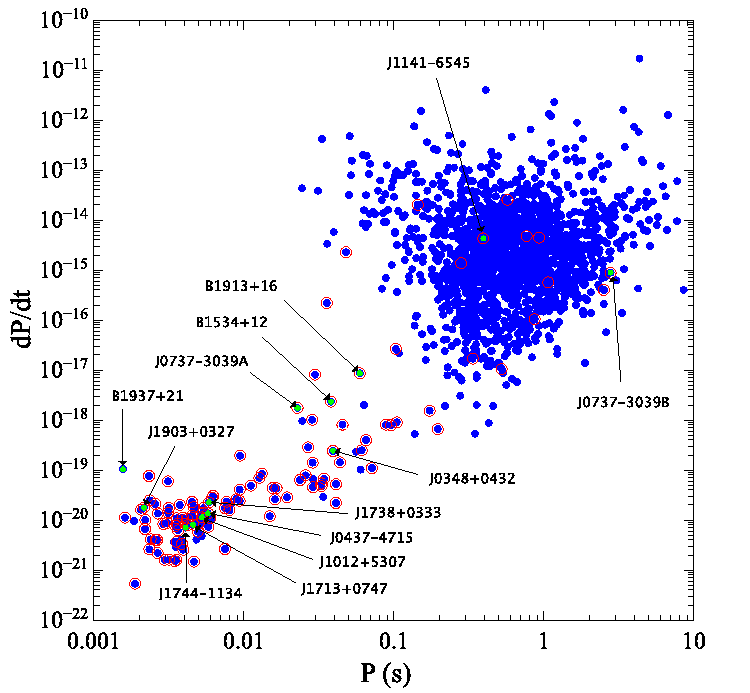
\includegraphics[width=\textwidth]{./figures/fig_P_Pdot_with_names.png}
\end{figure}


A gravitational wave is a perturbation in spacetime caused by a rotating
mass quadrupole moment somewhere in the universe. The most common sources of gravitational
waves are black hole binary systems, especially supermassive ($10^9$ solar
masses or more) black hole binaries
that occur in association with galaxy collisions. Such binary systems emit sinusoidal
GWs that give rise to the perturbation.
This perturbation occurs in the local metric of the space, and represents a
change in the space-time intervals between objects. The co-ordinate distances
remain fixed, but the practical (e.g. light travel time) distance is perturbed
slightly.

The Laser Interferometer Gravitational-Wave Observatory (LIGO) detectors recently announced the first detection of gravitational
waves \cite{LIGO}. The experiment detected a strain $\frac{\delta L}{L} \approx 10^{-21}$, corresponding to an absolute
distance change on the order of a fraction of a proton diameter. The LIGO
observatory was able to detect such small changes in distance by using an
optimized interferometer. By splitting a laser along two orthogonal paths,
reflecting them back to each other, and observing the interference magnitude, an
interferometer is able to precisely measure extremely small changes in the
differential lengths of their arms. One way of conceptualizing the
interferometer is by following the peaks (highest electric field magnitude) of
the light emitted by the laser across the device. The peaks are evenly spaced
in the arm, and without loss of generality will recombine constructively.
However, imagine a change in the length of one of the arms. Now, the peaks
along one arm have more distance to travel, and thus will arrive delayed
compared to their companions. Such a delay will induce a slightly destructive
interference in the resulting recombination beam, and will be detectable by a
light intensity detector. One can think of the stable arm as a ``reference
beam'', and the changing arm as the ``detector beam''. With this mode of
thinking, the interferometer acts as a comparison device between the reference
beam and the detector beam.

In a way, pulsar timing functions the same way as interferometers do. The
line-of-sight between us and the pulsar functions as the detector beam, with the
pulses originating from the pulsar functioning as the crests. In order to get
the equivalent of a reference beam, it is necessary to develop a timing model
that describes with great precision the expected time of arrival of the pulse
from the pulsar. With such a timing model, it is possible to compare the
measured time of arrival and the expected time of arrival to gain information
about the distance changes along the line-of-sight of the pulsar.

However, such a method requires an incredibly accurate timing model for the
pulsar that takes into account all known effects between the earth and the
pulsar. Such a model has been developed, and is used in the analysis pipeline to
accurately calculate the expected time of arrival of a pulse. The timing model
takes into account a wide array of effects. First and foremost, the timing model
requires a precise measurement of the period of the observed pulsar, as well as
the spindown rate, to model the pulse source accurately. Next, the timing model
takes into account the motion of the earth relative to the pulsar. The model
normalizes the times of arrival to the center of the solar system, and accounts
for the movement of the pulsar towards, away, or transverse to the solar system.
Next, the model takes into account any effects due to general relativity,
including the Shapiro delay effect for binary systems, and precession for
orbiting pulsars. The Shapiro delay is a time dilation in a pulsar's pulsation
rate when those pulses pass near a massive object (in this case, the object
being the pulsar's binary companion).

The ultimate goal of the timing model is to ``zero out'' any known effects between
us and the pulsar. After the timing model is made, any deviation we observe from
the timing model must be due to some unmodeled effect.

At regular intervals, the North American Nanohertz Observatory for Gravitational
Waves (NANOGrav) observes the 49 pulsars that are in the pulsar timing array
using the Arecibo Observatory in Puerto Rico and the Green Bank Telescope (GBT)
in West Virginia. Such observations allow comparisons to be made between the
expected times of arrival and the measured times of arrival. One use of these
observations is to improve the timing model for the pulsar. Deviations from the
timing model that follow known patterns due to incorrect timing model values can
give insight on how to improve the timing model parameters.  Thus, the timing
model is ``self-correcting'' in the sense that observations themselves improve
the precision of the timing model (see Figure 2).

\begin{figure}
\caption{Having an incorrect parameter in the model produces easily detectable
    and correctable signatures in the residual data \cite{Lorimer2008}. The
    residuals plotted here represent the magnitude of deviation from the
    expected time of arrival.}
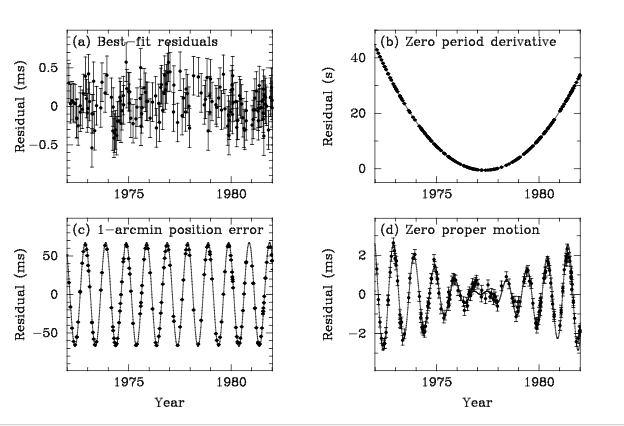
\includegraphics[width=\textwidth]{./figures/bad_timing.png}
\end{figure}


However, there may be deviations from the timing model that do not correspond to
incorrect parameters. These deviations must necessarily, then, come from
unmodeled processes. Of the most importance is the deviation corresponding to a
sine-like change in the distance between us and the pulsar. Although there could
be many potential sources for such a perturbation, a likely candidate is a
gravitational wave between the earth and the pulsar. It is possible, however,
that such a sine-like signal corresponds to an unmodeled process in the timing
model. For example, if the pulsar were in a binary system that was not known
beforehand, it would appear as if the distance between us and the pulsar were
changing sinusoidally because it actually is changing sinusoidally due to the
orbit of the pulsar around its companion! Many binary systems have been
discovered this way, long before optical telescopes verify the existence of
the companion.

To verify whether or not a sine-like signal corresponds to a gravitational wave,
the data is searched for a time correlation between pulsars. If the sine wave
shows up in multiple pulsars, then it can be concluded that the signal is not
originating from an unmodeled process in any individual pulsar. Such a
correlated signal must, then, correspond to some unmodeled process in the space
between all the pulsars in the galaxy. Using the relative locations of the
pulsars, specifics of the sine signal can be probed. Polarity and propagation
direction can be ascertained from the relative amplitudes of the signals in the
different pulsars in the pulsar timing array.

\section{Stochastic Detection}
While continuous wave sources are detectable by the PTA, the stochastic
background of GWs is what the PTA is best tuned for. The
stochastic background of GWs is the sum of all the gravitational
waves passing through our galaxy. Dominating the stochastic background is the
vast collection of GWs from supermassive black hole binaries.
Using the pulsar timing array, the properties of the stochastic background can
be probed. This is done by looking for correlated signals across the pulsars, in
an analysis similar to the continuous wave search method. By looking for these
correlated signals in the data, it is possible to ascertain the relative
abundance of the frequencies of waves that contribute to the background. This
data can be used, then, to reconstruct population statistics of black hole masses
and orbital frequencies in the universe. This gives information on galaxy
collision rates, as well as collision duration lengths and galactic black hole masses.

\section{High-Frequency Continuous Wave Detection}

The International Pulsar Timing Array (IPTA) is a consortium of collaborations
from around the world, including NANOGrav in North America, the European Pulsar
Timing Array (EPTA) in Europe, and the Parkes Pulsar Timing Array (PPTA) in
Australia. The IPTA is tuned to probe GW frequencies in the months-to-years
timescale. Observations of individual pulsars are carried out on a biweekly
basis, due to the large number of pulsars that need to be observed. With such
infrequent observations, however, GW frequencies on the order of hours remain
unexplored. This is due to the intrinsic limit on detection set by the Nyquist
frequency, defined as the maximum frequency periodic signal that is detectable
for a given sampling frequency. In order to accurately sample a periodic signal,
it is necessary to sample at least twice per cycle to avoid introducing errors.
Beyond this frequency, the sampling rate is not enough to properly detect a sine
wave signal, and any such CW signal would appear as white noise in the data.

Recently, a 24-hour global observation was carried out on J1713+0747, a particular pulsar, which
resulted in a new set of limits on continuous wave (CW) strain in the days to
hours frequencies due to the average sampling rate of about 0.5 samples/min
\cite{Dolch2016}.
Limits were set for both CW sources in the direction of J1713, as well as
random-direction CW sources.

  However, J1713 is not the only pulsar that has been observed for long,
continuous observations. The pulsars J2302+4442 and J0613--0200 were each observed for
multiple hours at a time at the GBT, originally for the purpose of measuring the Shapiro
delay effect for each of the pulsars (\cite{Pennucci2015}, \cite{Fonseca2016}). 
Such data sets (see Figures 3 and 4) allow for analysis similar
to that done to the J1713 24-hour campaign. These pulsars allow for better
directional limits to be placed in the microhertz to millihertz frequency range (Figure 5).

\section{Data Used}
 
\begin{figure}[h!]
    \caption{Timing residual plot for the three-hour observation of J0613--0200.
Integration time is 120s, and error bars are at the 1-sigma level. Data from
four separate sub-bands in the 820MHz band are plotted.}
    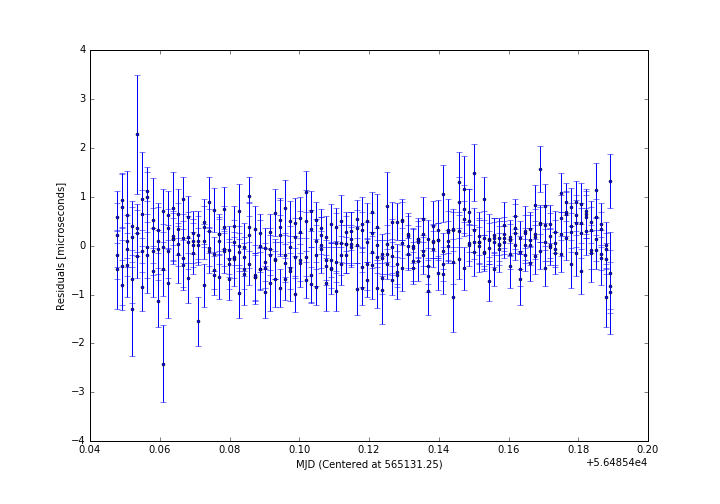
\includegraphics[width=\textwidth]{./figures/J0613_residuals.png}
\end{figure}

\begin{figure}[h!]
    \caption{Timing residual plot of the eight-hour observation of J2302+4442. The
integration time is 120s, and the error bars are at the 1-sigma level. Data from
four separate sub-bands in the 820MHz band are plotted.}
    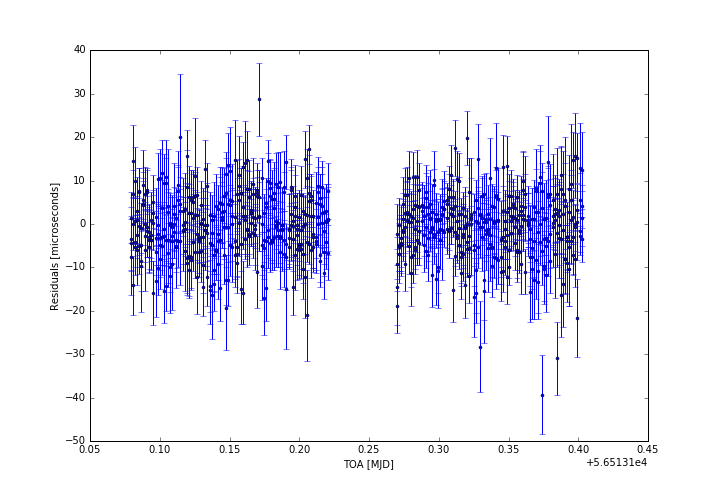
\includegraphics[width=\textwidth]{./figures/J2302_residuals.png}
\end{figure}

   In 2013, eight pulsars were observed for extended periods of time with the GBT for the
initial purpose of observing NANOGrav pulsars with significant Shapiro delays,
targeted strategically in order to better observe the delays and therefore
improve timing models (\cite{Pennucci2015}, \cite{Fonseca2016}). 
Of the eight data sets, two were chosen for our
analysis. Both J2302+4442 and J0613--0200 had small rms residual values, and
long continuous timing tracks.  Each pulsar was observed three times over the
course of the full observation period.  For each pulsar, the longest single
observation track was selected for observation. J2302 was observed continuously
for over 8 hours, and J0613 was observed continuously for over three hours.
The residuals were generated using the tempo2 software, drawing its parameters
from NANOGrav's 9-year data release. The binary orbit periods of each pulsar
are of particular interest, as a binary period naturally weakens the
sensitivity of the pulsar to continuous wave sources of a similar frequency.
The binary period for pulsar J2302 is given as about 126 days, and the binary
period for pulsar J0613 is given as about 1.2 days.

\begin{figure}[h!]
    \caption{Sky location in RA/DEC of the three pulsars analyzed (J0613--0200,
    J0645+5158, and
J2302+4442), as well as the previously-analyzed J1713+0747. Directional limits
    are placed in the directions of J2302 and J0645}
    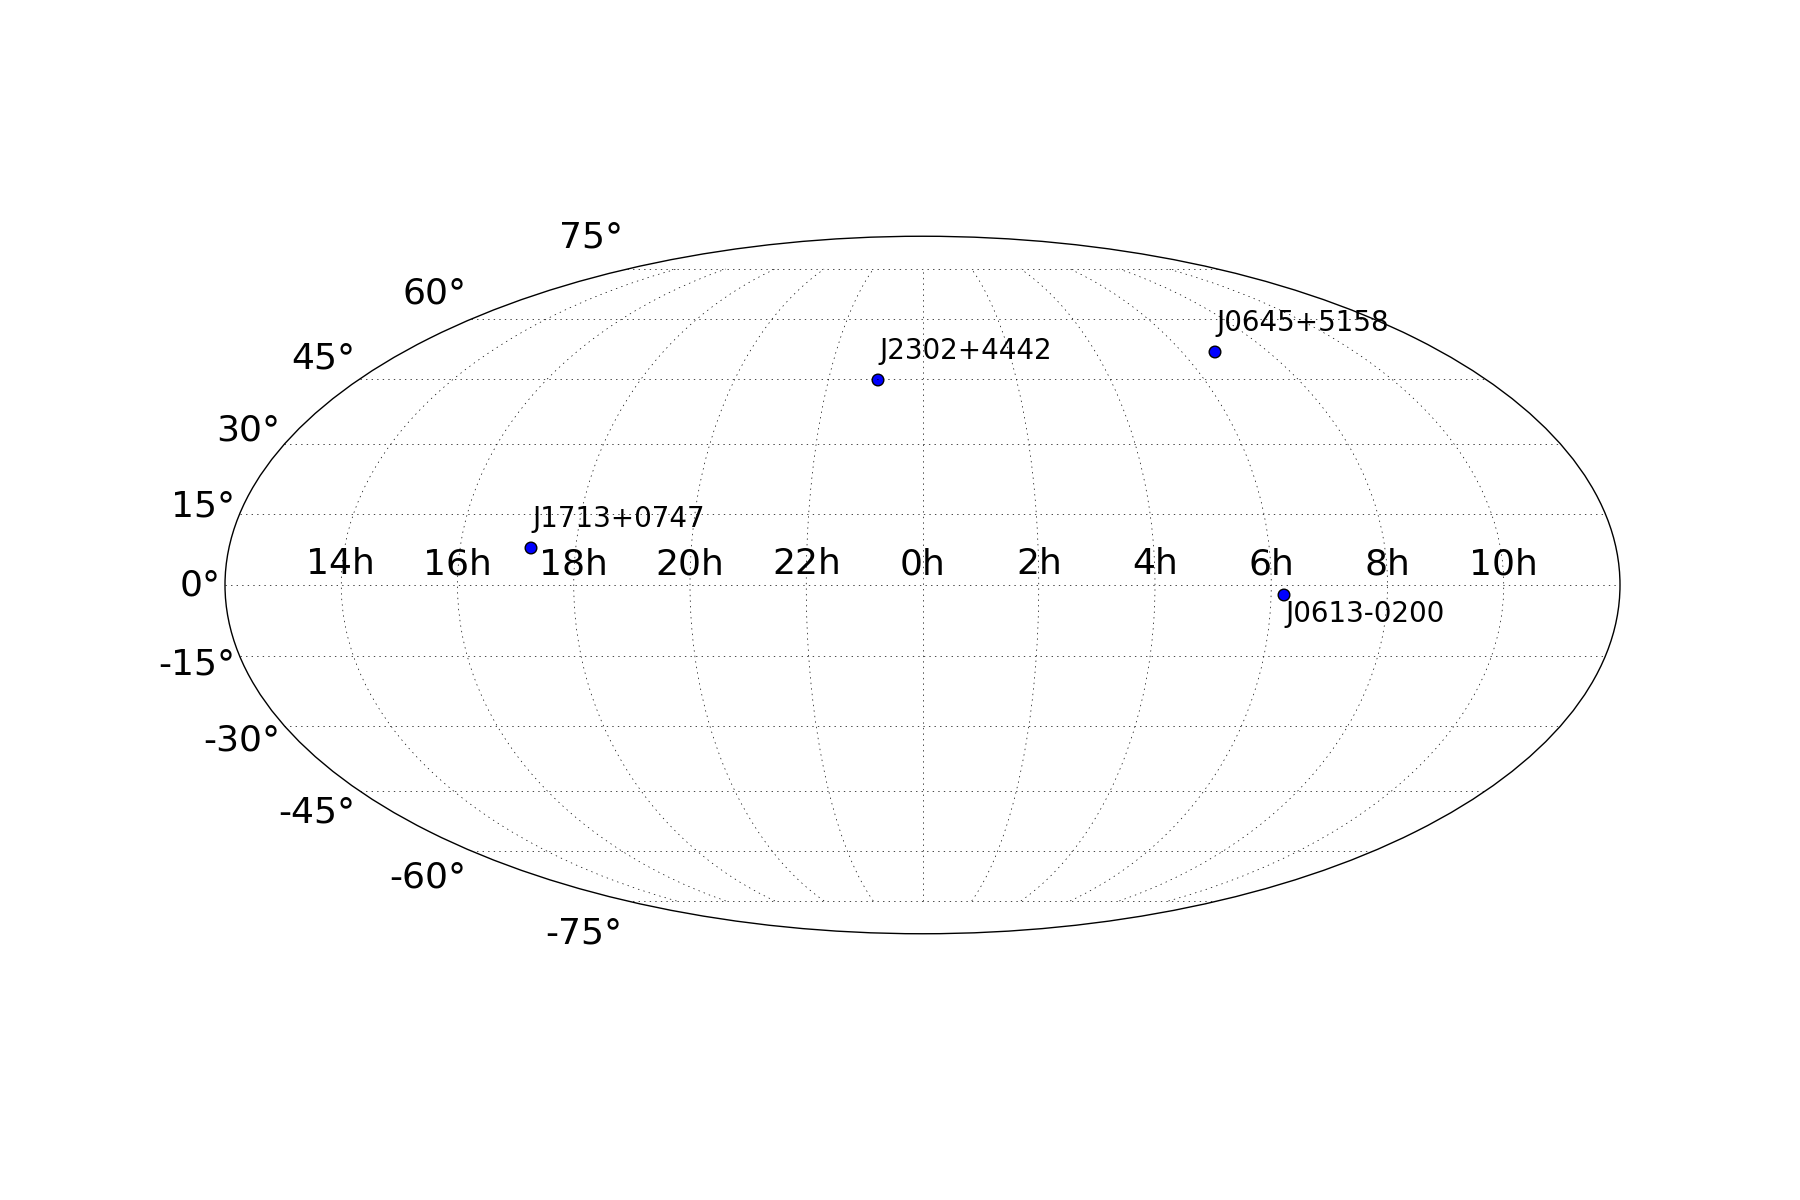
\includegraphics[width=\textwidth]{./figures/skyplot.png}
\end{figure}



\section{Data Analysis}
\subsection{Noise}
   For each pulsar, we developed a noise model to account for any intrinsic or
extrinsic sources of noise in the data. The model included both white and red
noise estimations. Five parameters were varied: EFAC, EQUAD, Jitter-EQUAD,
RN-Amplitude, and RN-Spectral-Index. Using the Markov Chain Monte Carlo method
for exploring parameter spaces, we found the maximum a posteriori values for
each parameter, and used them to construct the noise covariance matrix.

The five parameters were chosen for a noise model that has been used in
previous analysis schemes. The EFAC parameter acts as a constant multiplier on
the TOA uncertainties. The EQUAD parameters represent additional Gaussian white
noise added to the EFAC noise. The RN-Amplitude and RN-Spectral-Index parameters
describe a red noise variance. 

\subsection{Detection Statistic}

\begin{figure}[h!]
\caption{The $F_p$ statistic calculated from the residuals. The dashed line shows
    the minimum $F_p$ value needed to claim a detection with a false alarm probability
    of 1e-4.}
\includegraphics[width=\textwidth]{./figures/both_fp_presentation.png}
\end{figure}

    Our main tool for analyzing the sensitivity of a pulsar to continuous wave
sources is the $F_p$ statistic (\cite{Arz2014}). The
$F_p$ statistic is a frequentist detection statistic. It can be thought of as a
measure of how much a particular frequency dominates the data. A high $F_p$
statistic is indicative of a potential CW source at that frequency. For each
potential CW frequency, we calculate the $F_p$ statistic for the data at that
frequency. Our detection threshold of about $F_p \geq 13$ corresponds to a false
alarm probability of $10^{-4}$. That is, the probability of data with an $F_p$
statistic above the minimum value being realized purely by noise (and not a
signal) is one in ten thousand.

\subsection{Upper Limits and Source Simulation}

After creating the noise model for the pulsar, we determine the sensitivity to
CW sources at different gravitational wave frequencies. On a high level, this
is done by simulating CW sources in random directions with a given strain, and
seeing if they can be detected with the given noise model. By ramping up the
simulated strain until a detection is made, we obtain the lowest detectable
strain--the strain limit--for that GW frequency. To determine whether or not a
specific strain can be detected, we simulate 50,000 sources sequentially in
either random directions or, in the case of a directional search, in the
direction of the pulsar. Each source is simulated with a random GW emission inclination,
and a set distance to keep the strain amplitude constant. Then, for each
source, we create simulated residuals based on the CW source and the noise
model, and generate an $F_p$ statistic. A source is labelled ``detectable'' if the
$F_p$ statistic is higher than the actual data's $F_p$ statistic. If more than 95\% of
the simulated sources are detectable, then it can be concluded that a CW source
with a strain equal to the fixed strain is detectable above the noise. Thus,
that strain is an upper bound on CW source strains for the particular GW
frequency being examined.

\section{Results}

\begin{figure}
    \caption{Recent single-source GW limits from the PPTA, EPTA, and NANOGrav,
as well as single-pulsar limits from J0437-0745 and B1937+21. Also plotted is
the high frequency limits obtained in this analysis from J0613--0200,
    J0645+5158, and
J2302+4442, and the previously published limit from J1713+0747. Here, the data
    from the Beklen campaign was used for J0613}
    \includegraphics[width=1\textwidth]{./figures/all_limits_incfall.png}
    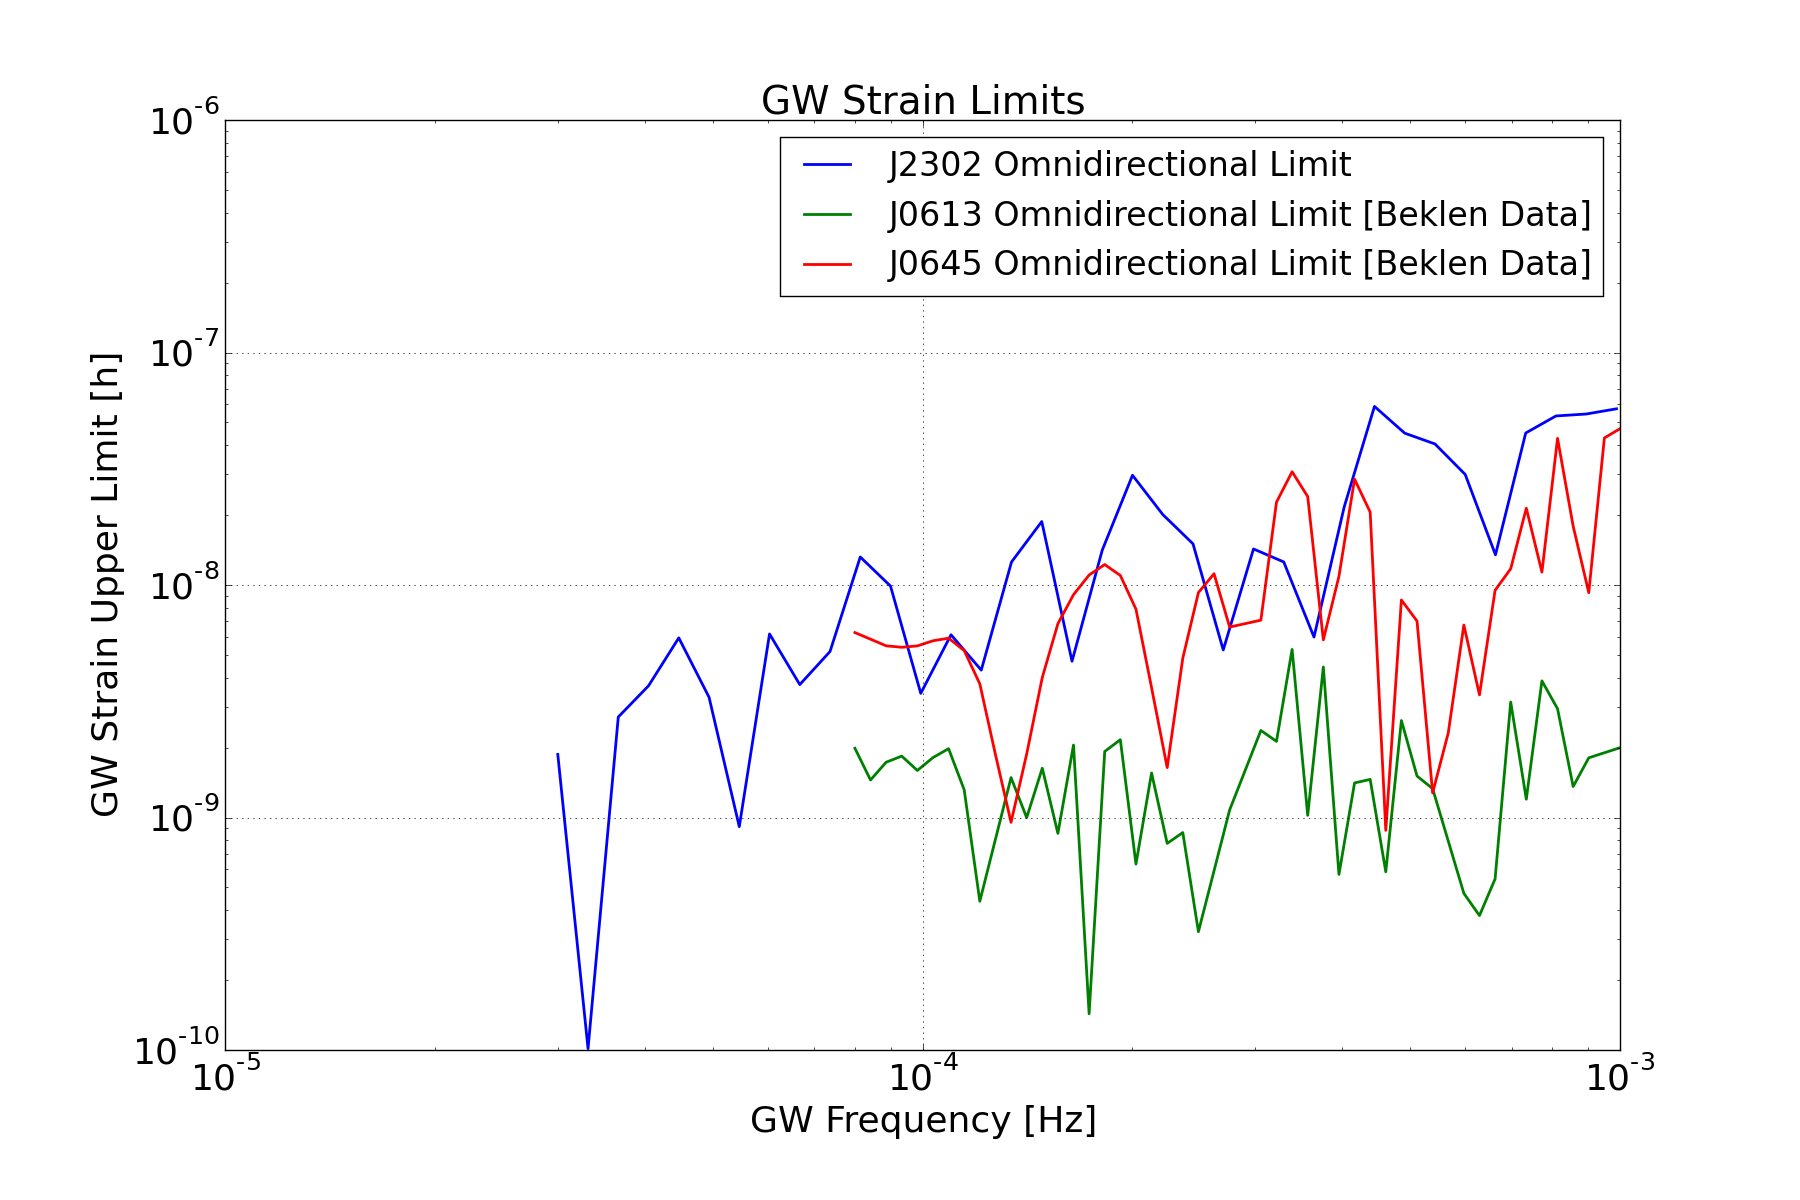
\includegraphics[width=1\textwidth]{./figures/hf_limits.png}
\end{figure}

Applying the $F_p$ statistic algorithm to the two pulsars analyzed, we found
there was no evidence for a single source gravitational wave signal. However,
using the source simulation algorithm, we were able to place upper limits on the
strength of the GWs passing through the galaxy at the
frequencies probed. Such limits were in coincidence with previously published
limits from pulsar J1713+0747. Furthermore, the results coincide with a
reasonable extrapolation of the results obtained by NANOGrav and the other PTA
consortia.

\subsection{Pulsar J0613-0200}

Data from the Pennucci campaign (\cite{Pennucci2015}), and the Beklen campaign on PSR J0613-0200 had the
smallest average error bars at around 1 microsecond. However, the pulsar is in a
binary orbit with period of just over one day, which lies very close to the
range of frequencies probed in this study. For this reason, the upper limit
curve turns over at low frequencies, as any GW signal could be confounded with
an error in the binary period.

Ultimately, the data taken by Beklen had better noise modeling, and produced the
lowest omnidirectional limit curve. While this limit curve did not supersede the
previously published J1713 limit curve at all frequencies, it lies within an
order of magnitude of the J1713 limit.

The precision of the timing of J0613 is reflected in the $F_p$ plot, as J0613
has the smallest $F_p$ statistic, corresponding to more certainty in the
non-detection of a signal.

\subsection{Pulsar J0645+5158}

Pulsar J0645+5158 was observed by Elif Beklen on the Green Bank telescope, and
offers the best limits in both the omnidirectional and directional cases. Since
J0645 is not in a binary system, we do not have the same problem that J0613 has
with binary period conflation. However, due to larger error bars, J0645 was not
able to match J0613 in the omnidirectional limit curve.

However, J0645 was able to produce the best directional limit curve. The
directional limit was about one order of magnitude lower than the
omnidirectional limit, which matches with the behavior of the J1713
omnidirectional and directional limits. 

An interesting feature of the J0645 data lies in the structure of the
low-frequency limit curve. Certain features, such as the parabolic sweep near
the tail end, appear in both the directional and omnidirectional limit curves.
This suggests some structure to the residuals that may have been unaccounted for
in the noise modeling. Such structure is not explored in this work, but may be
the topic of study for future work.


\subsection{Pulsar J2302+4442}

Pulsar J2302+4442 was observed in the Pennucci campaign, and is the longest data
set analyzed. The campaign took data for eight hours, which allows analysis for
detection of GWs at periods up to eight hours in length. For this reason, J2302
provides the most comprehensive limit, extending almost an order of magnitude in
frequency beyond the other pulsars analyzed.

J2302 also provided good directional limits, which again were consistently about
an order of magnitude below the corresponding directional limit.

\begin{figure}
    \caption{Directional limits established in the direction of J2302 and J0645.
    Also plotted is the J0613 directional limit from the Beklen campaign, which was significantly higher
    than expected.}
    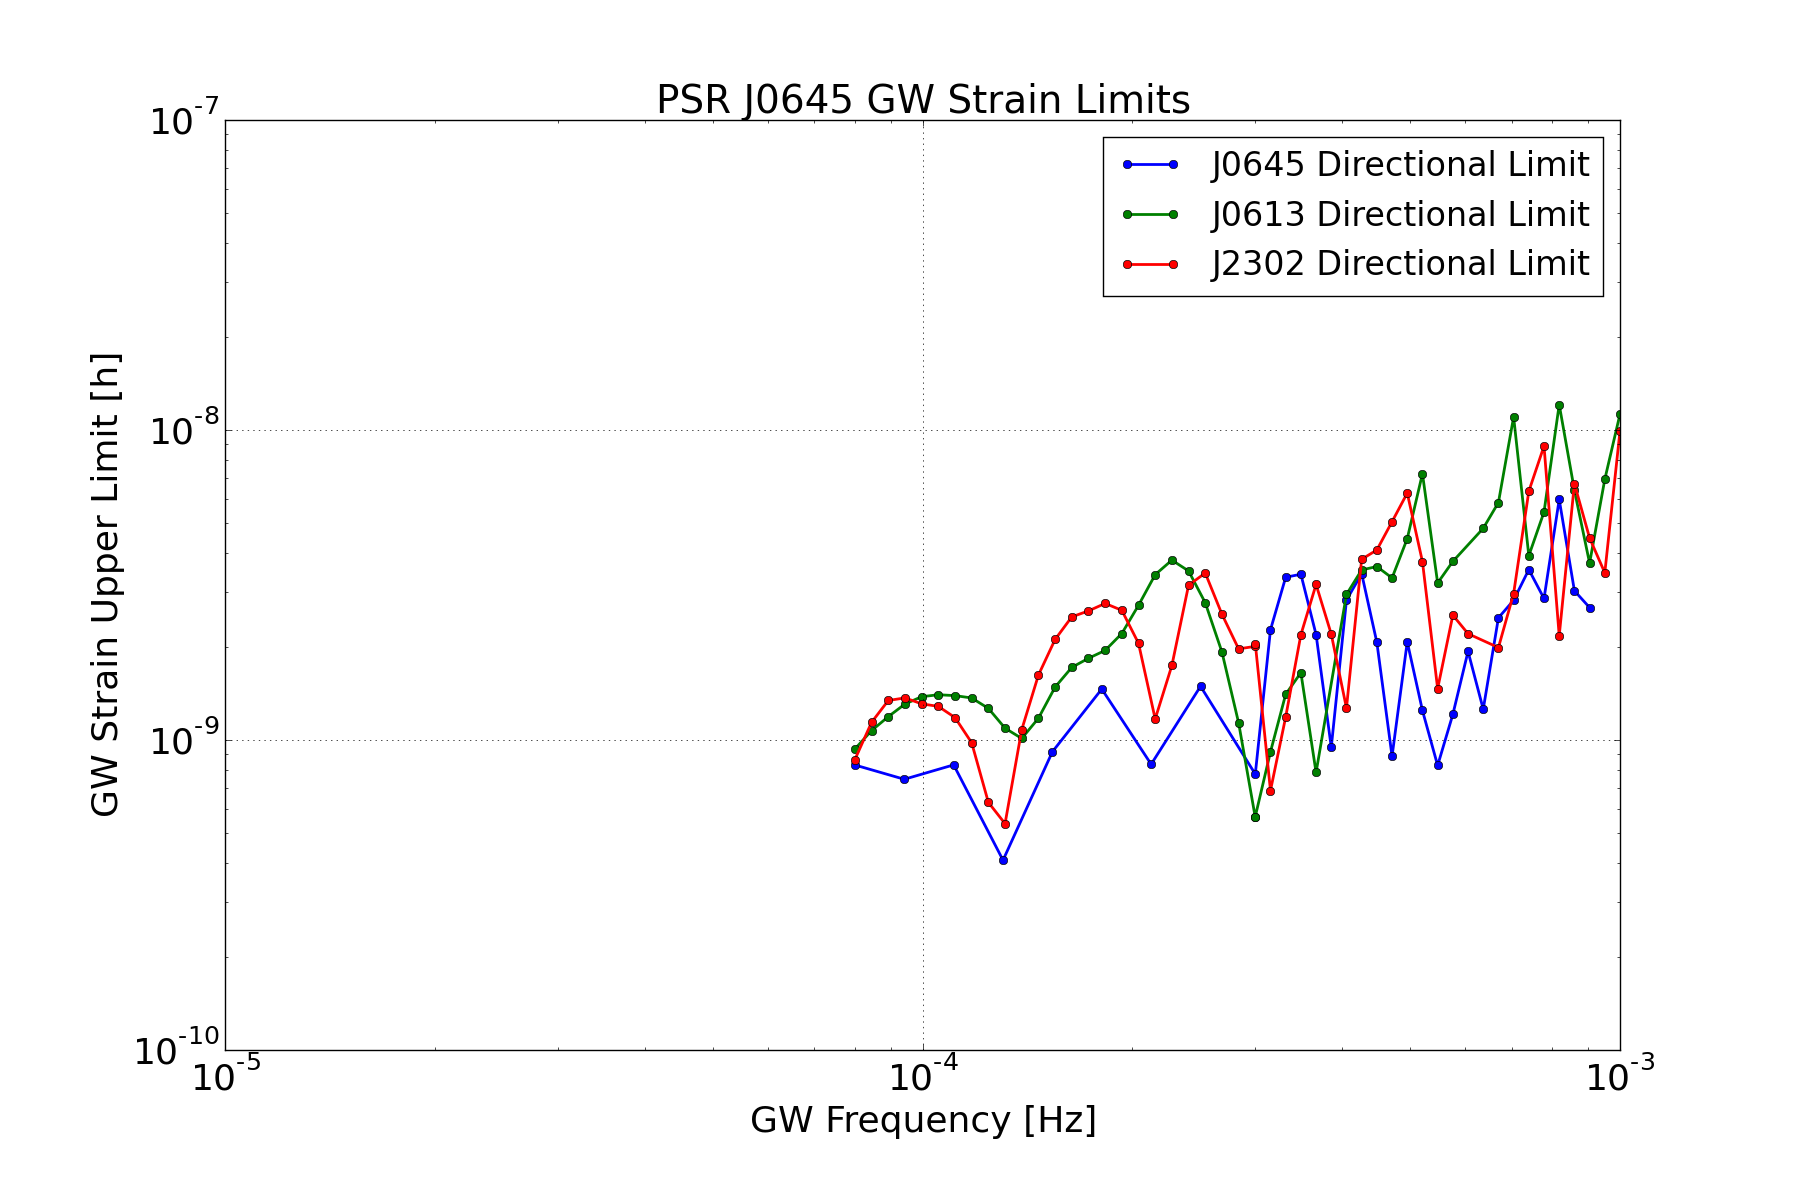
\includegraphics[width=1\textwidth]{./figures/all_directional.png}
\end{figure}

\section{Conclusion}
    Using our pipeline, we were able to recreate the omnidirecitonal limits from the J1713 24-hour global campaign, which verified the
integrity of our analysis algorithm. Using data from the Green Bank Telescope
taken by Tim Pennucci and Elif Beklen on puslars J0613-0200, J0645+5158, and
J2302+4442, we
were able to place omnidirectional limits consistent with limits already placed
in that GW frequency range. 
    Furthermore, directional limits in the direction of pulsars J0645 and J2302
    were placed, which limited GW strains by an additional order of magnitude in
    these directions.

    Further analysis will attempt to remove statistical fluctuations in the data
through using a greater amount of simulations. Furthermore, the noise model can
be improved upon by sampling the parameter space of the noise model more
precisely. Also, similar analyses can be carried out on each of the other
pulsars observed in the two projects. For
each pulsar, strict directional limits on CW strain amplitude can be placed for
GW frequencies in the microhertz to millihertz range.

The directional limit curve for J0613 did not follow the pattern of being
reduced by an order of magnitude. Instead, the directional limit was worse than
the omnidirectional limit. This result is very surprising, and indicates a
problem in the noise model for J0613. Further study of the noise model for this
pulsar will shed light onto the nature of this discrepancy.

This method, however, is not the only way to probe the microhertz to millihertz
frequency range. The Laser Interferometer Space Antenna (LISA) will be sensitive
to these frequencies as well, and will have much better sensitivity. However,
the lines-of-sight of LISA will be very localized (~1000km) compared to the
lines-of-sight of the PTA, which extend across the galaxy. For this reason, PTAs
are very sensitive to galactic-source objects that may fall in a line-of-sight.
In this scenario, the apparent strain for the PTA will be much larger than the
apparent strain for LISA, and the PTA will have a better chance at detecting
these sorts of sources. Work is being done to modify the PTA analysis for
intragalactic source detection and limit generation, but such calculations
require strong-field relativity, which is much more difficult to work with.

\section*{Appendix A}

Step-By-Step Instructions for Data Analysis of Long-Track Data for High
Frequency GW Detection

What you'll need: -computer with linux installed (could potentially work on mac
as well)

\subsection*{Installing tempo2}

Tempo2 can be found at
\url{https://bitbucket.org/psrsoft/tempo2}, or grabbed by using the command

\begin{lstlisting}[language=bash]
git clone https://bitbucket.org/psrsoft/tempo2.git
\end{lstlisting}

After getting all the files, follow the instructions included in the README.
[Plugins like plk (the graphics interface that uses PGPLOT) are not necessary for
data analysis, but can be useful to visualize your data before analysis.
However, installation of PGPLOT and plk is not covered in this manual.]

The command ./configure will attempt to configure all compilers and plugins to
get ready for the make. Any errors you might have will come up in this step.
Note, if you would like to install tempo2 in a particular location aside from
the default, use the command
	
\begin{lstlisting}[language=bash]
./configure --prefix=/your/install/path
\end{lstlisting}

If you are getting an error regarding your gcc and F77:
Make sure you have compilers for c and fortran installed, since tempo2 requires
both of them. Furthermore, they need to be able to cross link.
Some versions of F77, for example, do not cross link with other versions of gcc.
Therefore, it is best to use gcc and gfortran to compile tempo2. If
\texttt{./configure}
is still looking at F77 instead of gfortran, run the command

\begin{lstlisting}[language=bash]
export F77=gfortran
\end{lstlisting}

Which will set your fortran compiler to gfortran manually. Then, run
\texttt{./configure}
again to pick up the changes.

Once \texttt{./configure} passes, the environment is set up to run make correctly.
Running the command

\begin{lstlisting}[language=bash]
make && make install
\end{lstlisting}

will compile all the necessary components. Note, you may have to run as su, as
make creates some new directories.

That's it! You can run make clean to delete the unnecessary files from
installation, and you can run \texttt{make plugins \&\& make install plugins} to install
the relevant plugins. 

If everything worked successfully, there should now be a program called tempo2 that
is runnable from the command line. Running 

\begin{lstlisting}[language=bash]
tempo2 -v
\end{lstlisting}

will verify that tempo2 is correctly installed.

\subsection*{Installing PAL2}

Luckily, PAL2 is significantly easier to install than tempo2.
First, clone the git repo with the command
\\
\begin{lstlisting}[language=bash]
git clone https://github.com/jellis18/PAL2.git
\end{lstlisting}

Second, you'll want to grab an environment manager like Anaconda
(\url{https://docs.continuum.io/anaconda/install}) to manage the python packages that
PAL2 needs. After installing anaconda, run the command
\\
\begin{lstlisting}[language=bash]
conda env create -f environment.yml
\end{lstlisting}
which will create an environment called \texttt{pal2\_conda} based off the dependencies in
\texttt{environment.yml}. Note, if there are issues with certain versions not being
available for your OS, use the command 
\\
\begin{lstlisting}[language=bash]
conda search \$PACKAGE
\end{lstlisting}
where \texttt{\$PACKAGE} is the package name that has an incompatible version, and find
the version number that is closest to the one \texttt{environment.yml} wants. Then, edit
\texttt{environment.yml} to the version numbers that work.
	
After conda creates the environment, switch to it with 
\\
\begin{lstlisting}[language=bash]
source activate pal2\_conda
\end{lstlisting}

Next, proceed with the installations that conda does not handle with the
commands
\\
\begin{lstlisting}[language=bash]
pip install -r requirements.txt
pip install libstempo --install-option="--with-tempo2=\$TEMPO2"
\end{lstlisting}
and run
\\
\begin{lstlisting}[language=bash]
python setup.py install
\end{lstlisting}

If everything worked successfully, the scripts \texttt{makeh5File.py} and
\texttt{PAL2\_run.py} should
be executable. Check this with:
\\
\begin{lstlisting}[language=bash]
./PAL2\_run.py -h
\end{lstlisting}
If the installation was successful, the script should return a long list of
options that are available.


\subsection*{Generating an hdf5 file}

In order to properly process the data from a .par and .tim file, it must first 
be put into a format that PAL2 can handle. The hdf5 format (Hierarchical Data
Format 5) was chosen as the data model to store the relevant data from the .par
and .tim files.
In order to convert raw data into an hdf5 data model, the data must first be
consolidated into a single .tim file with a single .par file to go with it. The
.par should have fits turned on for FD parameters, as well as DM and F0.
Put the .tim file in a subdirectory (usually \texttt{./tim/}) and the .par file in a
different subdirectory (usually \texttt{./par/}). Then, run the \texttt{makeH5File.py} script that
came packaged with PAL2.
\\
\begin{lstlisting}[language=bash]
makeH5File.py --pardir "./par/" --timdir "./tim/"
--h5File "name\_of\_output.hdf5"
\end{lstlisting}

If everything worked successfully, there should now be a file called
\texttt{"name\_of\_output.hdf5"} in the current directory. This is the file to send to the
upper limit script.

\subsection*{Generating Noise}

In order to correctly run simulations based on the data, a proper noise model
must be established. This is done by exploring the noise model parameter space
(usually a five-dimensional space) using a Markov Chain Monte Carlo algorithm to
maximize the likelihood that a particular combination of parameters models the
noise correctly. To run the algorithm, invoke the \texttt{PAL2\_run} script with:
\\
\begin{lstlisting}[language=bash]
PAL2\_run.py --h5File "/path/to/h5File.hdf5" --outDir
"/path/to/output/directory/" --nf 30 --incEquad --incJitterEquad
--mark6 --pulsar <pulsar name>
\end{lstlisting}

The additional parameter \texttt{--incRed} will include two additional parameters for
modelling red noise, but may not be necessary for short data sets.

If everything worked successfully, there should now be a directory with the
noise data stored in multiple .txt files. The specific format of the noise
subdirectory is not important, as the upper limit script knows how to deal with
it.

\subsection*{Generating an Upper Limit}

Once the noise model is built correctly, the final step is to run the suite of
simulations in the \texttt{generateUpperLimit.py} file for the data and noise model. This
can be done by running the command:
\\
\begin{lstlisting}[language=bash]
generateUpperLimits.py --file /path/to/hdf5File.hdf5
--noise-dir /path/to/noise/ --out-dir /path/to/output/directory/
--psr <pulsar name> --frq-resolution 50 --nreal 10000
--run-name <descriptive simulation name>}
\end{lstlisting}

The parameter \texttt{--frq-resolution} can be changed to sample the frequency window
more or less depending on how resolved you need the limit curve to be. The
parameter \texttt{--nreal} controls the number of realizations (or simulations) done per
upper limit. It should be no less than 10000, and in practice should be a lot
more than that.

The script will output its results per-frequency to stdout, as well as to a text
file that it will generate and save in the \texttt{--out-dir}. 

If everything worked successfully, there should now be a numpy-compatible .txt
file with the generated upper limit on CW strain in the frequency range
specified in \texttt{generateUpperLimit.py}!

\newpage

\nocite{*}

\bibliography{laureates_references}

\bibliographystyle{abbrv}

%\newpage
%\section*{Bibliography}
%Astrophysical Journal, 794, 141
%\\
%\newline\noindent Dolch, T., NANOGrav Collaboration, Ellis, J.~A., et al.\ 2016,
%Journal of Physics Conference Series, 716, 012014
%\\
%\newline\noindent Fonseca, E., Pennucci, T.~T., Ellis, J.~A., et al.\ 2016, arXiv:1603.00545 
%%\newline\noindent
%\\
%\newline\noindent Lorimer, D.~R.\ 2008, Living Reviews in Relativity, 11
%\\
%\newline\noindent Pennucci, T.~T.\ 2015, Ph.D.~Thesis
%\\
%\newline\noindent Abbott, B. et al.\ 2016 Phys. Rev. Lett., 116, 061102
%
\end{document}
